\documentclass[14pt]{article}
\usepackage{geometry}                % See geometry.pdf to learn the layout options. There are lots.
\geometry{a4paper}                   % ... or a4paper or a5paper or ... 

\usepackage[parfill]{parskip}    % Activate to begin paragraphs with an empty line rather than an indent
\usepackage{fullpage}
\usepackage{graphicx}
\usepackage{grffile}
\usepackage{listings}
\usepackage{hyperref}
\usepackage{tabularx} %tabular with stretch columns
\usepackage{enumerate}
\usepackage{pdfpages}
\usepackage{pdflscape}
\usepackage[utf8]{inputenc}

\usepackage[acronym]{glossaries} % make a separate list of acronyms
\makeglossaries

% Index
\usepackage{makeidx}
\makeindex

\begin{document}

\begin{titlepage}

\begin{minipage}{4cm}
\begin{tabular}{l}

\includegraphics[width=0.5\textwidth]{Images/uppsala}
\end{tabular}
\end{minipage}
\hfill
\begin{minipage}{4cm}
\begin{tabular}{r}

\includegraphics[width=0.5\textwidth]{Images/logo}
\end{tabular}
\end{minipage}


\begin{center}
% Upper part of the page

\textmd{HealthShare Final Report}
\vfill
% Title
 \huge{\textbf{A Study on Methods to Increase Interoperabilty and Unify Electronic Healthcare Records } }\\[2.0cm]
for\\
\large\textbf{Uppsala County Council}\\[1.0cm]
by\\
\large{\textbf{Uppsala Universitet}} and \large{\textbf{Rose-Hulman Institute of Technology}}\\[1.0cm]

\end{center}

\begin{center}
\vfill
December 2011\\
\end{center}

\end{titlepage}

\begin{abstract}

\newglossaryentry{interoperability}{name={Interoperability}, description={The ability of diverse systems and organizations to work together. Please see section~\ref{sec:interopDefinition} for the meaning within health care}}

\newglossaryentry{Health Care Provider}{name={Health Care Provider}, description={an individual or an institution that provides health care services in a systematic way}}

\newacronym[\glsshortpluralkey=HCPs ,\glslongpluralkey= Health Care Providers]{HCP}{HCP}{\gls{Health Care Provider}}

\newglossaryentry{Swedish Association of Local Authorities and Regions}{name={Swedish Association of Local Authorities and Regions}, description={represents the governmental, professional and employer-related interests of Sweden's 290 municipalities and 20 county councils which include the regions of Gotland, Halland, Västra Götaland and Skåne}}

\newacronym{SALAR}{SALAR}{\gls{Swedish Association of Local Authorities and Regions}}

\newglossaryentry{Center for eHealth in Sweden}{name={Center for eHealth in Sweden}, description={governed by representatives of county councils and regions, \gls{SALAR}, municipalities and private care providers}}

\newacronym{CeHis}{CeHis}{\gls{Center for eHealth in Sweden}}

\newglossaryentry{Electronic Medical Record}{name={Electronic Medical Record}, description={a digitalized, systematic documentation of a single patient's medical history and care across time within one particular \gls{HCP} jurisdiction}}

\newacronym[\glsshortpluralkey=EMRs ,\glslongpluralkey= Electronic Medical Records]{EMR}{EMR}{\gls{Electronic Medical Record}}


\newglossaryentry{Electronic Healthcare Record}{name={Electronic Healthcare Record}, description={an \gls{EMR} or a collection of \glspl{EMR} that can be shared across networks between different \glspl{HCP}}}

\newacronym[\glsshortpluralkey=EHRs ,\glslongpluralkey= Electronic Healthcare Records]{EHR}{EHR}{\gls{Electronic Healthcare Record}}

\newglossaryentry{Personal Health Record}{name={Personal Health Record}, description={a health record where health data is maintained and owned by the individual it pertains to, rather than an institution or a hospital}}

\newacronym[\glsshortpluralkey=PHRs ,\glslongpluralkey= Personal Health Records]{PHR}{PHR}{\gls{Personal Health Record}}

\glspl{EHR} are rapidly expanding in their use and their benefits are well known. Significant reduction in the cost of care, improved quality of care, and improved record keeping are just a few of the benefits of using an \gls{EHR}. It is for these reasons that many medical institutions are rapidly adopting \glspl{EHR}. 

An explosion of innovation has stemmed from this rapid adoption and has produced many different solutions from many different providers. Unfortunately, these solutions tend to store and transmit the information that they collect in formats that are not compatible with each other. In order to maximize the benefit received from these \glspl{EHR} they must be able to share information between different systems and locations.

This paper reports on the various aspects of achieving \gls{EHR} \gls{interoperability}.
\end{abstract}

\newpage

\tableofcontents

\newpage

%\section*{Temporary section: How to do Glossary Entries}
%
%Look at the {\LaTeX} for the Abstract section to see how add glossary entries and how to use them in the text.
%
%An \gls{interoperability} entry and \gls{EHR}. Second use: \gls{EHR}.
%
%%Plurals: \glspl{interoperability}. 
%Reset acronym\glsreset{EHR}. \\
%Plural: First use: \glspl{EHR}. Second use: \glspl{EHR}.

\section{Introduction}
\label{sec:Introduction}

\subsection{Background}
Hospitals within Sweden use electronic computer systems to store and track patient health data. Different hospitals or medical facilities use systems developed by different companies or different customized solutions from the same company. The end result is a complex network of systems that are unable to communicate with each other. When a patient moves or visits a hospital while on vacation the individual doctors must manually send patient data to each other. This is a complicated and error-prone process that potentially wastes the time and energy of everyone involved.

%Define the problem and in what context (maybe contextualize, write a story, describe a scenario? a concrete relevant scenario that occurs with persons involved)

%The setting of problems in \gls{EHR}/EMR \gls{interoperability} situations. Describe what the problems related to \gls{interoperability} are within healthcare. The situation in Uppsala County, why we are doing this. What is being done on \gls{interoperability} in other areas. Describe the problems related to interoperating \glspl{EHR}.

%Describe the ideal interoperating system

\subsection{Purpose and Scope}
A world wide problem in medical records is to efficiently share patient medical records. Many patient records are electronically stored and the potential exists to make them accessible to patients and doctors using different systems. Enabling the sharing of \glspl{EHR} on a large scale could improve the treatment patients receive by increasing the information doctors have access to when they make medical decisions. With the ability for nurses and doctors to read a patient's medical history from a different \glspl{EHR} system they could potentially increase the speed and accuracy of treatment. There are also many obstacles associated with this initiative, such as ethical, legal and behavioral.

The HealthShare project conducted interviews and research into \gls{EHR} development in Europe and the Unites States over the past three months for the purpose of understanding the issues associated with building more successful, widespread \glspl{EHR} in the future. By inspecting current systems and talking to experts in the \gls{EHR} field, the project team worked to analyze the tremendous amount of \gls{EHR} knowledge and form a focused picture of a successful path to follow. Perhaps most essential to the development of \glspl{EHR} is the issue of interoperability. HealthShare specifically devoted many resources towards researching the intricate relationship between interoperability and \gls{EHR} systems. The lack of knowledge of this relationship has ruined many past \gls{EHR} projects and is of the utmost importance for progress in this sector of medicine.


\subsection{Reading Instructions}
Depending on your background, some portions of this document may be redundant or not applicable. This represents a best guess of what the authors feel would be the most relevant sections for different audiences.

These are, of course, just suggestions and you are free to read whatever sections you wish.

\begin{description}
\item[Administrators] Read the section on interoperability~\ref{sec:Interoperability} (focus on ~\ref{sec:interopSolutions} and ~\ref{sec:interopPrereq}). Skip the section on technical standards unless you are interested. Section ~\ref{sec:Future} focuses on the adoption of a future system, read ~\ref{sec:futureLegal}-~\ref{sec:futureUsability} about the non-technical issues. The results section is very important, focus on ~\ref{sec:resultsPrereq} and ~\ref{sec:resultsEndUser}. Section ~\ref{sec:Conclusions} describes the conclusions, read this.
\item[Doctors] Read section ~\ref{sec:peopleDirect}. Read section ~\ref{sec:interopCurrent}-~\ref{sec:interopPlans} to understand the current situation and possible solutions.~\ref{sec:TechnicalStandardsTerminology}-~\ref{sec:TechnicalStandardsAlternative} describes what we see as the optimal solution. Section ~\ref{sec:futureLegal}.-~\ref{sec:futureUsability} describes the non-technical issues with a future system. In the results section focus on ~\ref{sec:resultsEndUser}-~\ref{sec:resultsSecurity} and ~\ref{sec:resultsUsabilityTesting}.
\item[Politicians] Read section ~\ref{sec:People} which focuses on the users and stake holders. Read section ~\ref{sec:Interoperability} as well, focus on ~\ref{sec:interopPrereq} which describes the prerequisites for international interoperability. Read section ~\ref{sec:futureLegal}-~\ref{sec:futureUsability} which describes the non-technical issues with a future system. Read section ~\ref{sec:resultsPrereq} in the results section, also read the conclusions in section ~\ref{sec:Conclusions}.
\item[Public] Section ~\ref{sec:Interoperability} describes the current situation and defines interoperability, read ~\ref{sec:interopIntro} to ~\ref{sec:interopPrereq}. Read ~\ref{sec:technicalStandardsWhatIs}-~\ref{sec:technicalStandardsCreation} to understand what a standard is. Read sections ~\ref{sec:futureTechnical}-~\ref{sec:futureUsability} to understand the issues with a future system. In the results section read ~\ref{sec:resultsPrereq}-~\ref{sec:resultsEndUser}. The conclusions in section ~\ref{Conclusions} are relevant so read this section.
\item[Technicians] Section ~\ref{sec:Interoperability} and ~\ref{sec:TechnicalStandards} are very relevant since they describe the interoperability standards as well as the technical standards than can be used. Section ~\ref{sec:futureTechnical} describes the technical limitations of a future system, read this as well. The result section ~\ref{sec:Results} is very important, read the entire section, also read the conclusions in section ~\ref{sec:Conclusions}.

According to the technician's point of view \cite{FarzinYazdi}, the importance of interoperability between \glspl{EHR} is high because it is easier to exchange information between \glspl{EHR} when those are connected together \cite{FarzinYazdi}. If \glspl{EHR} are not connected to each other, there is risk for staffs to do their job twice in order to complete their tasks i.e. they should copy the original patitent data from primary \gls{EHR} to the secondary \gls{EHR} \cite{FarzinYazdi}. In other words they should do this task manually and there is risk for mistakes and it will take longer time comparing to the \glspl{EHR} that are connected to each other \cite{FarzinYazdi}.

At Karolinska hospital in Sweden, the employees use three different \glspl{EHR} which are neither not connected to each other nor those are not connected to the analyzer machines (the machines are online) \cite{FarzinYazdi}. This makes the work much harder and confusing because they have to decide which \gls{EHR} to choose. This working routine will result in many incorrect data registration. Since analyzer machines are not connected to \glspl{EHR} then technicians are not able to validate analyzed samples. The validation must be done manually and the result also must be written manually in \gls{EHR}\cite{FarzinYazdi}.  It is natural that a connection between the \glspl{EHR} will decrease incorrect data registration. The employees at Karolinska hospital in Sweden are very much aware about this problem \cite{FarzinYazdi}.

In Denmark, the new system didn't integrate with the old system at all. All the data from the old system were preserved and could not be reached in the new system \cite{FarzinYazdi}. The analyzer machine is connected to \gls{EHR} and the result will be saved automatically in \gls{EHR} \cite{FarzinYazdi}. The fact that new system has completely different platform made it harder to work with \cite{FarzinYazdi}.

One of the big problems that technicians are faced with it, is that sometimes confusions occur when two different employees with different backgrounds exchange information i.e. an employee doesn't know the code of the examination and he/she only knows the proper name of analyze but the name is unknown for other staffs so in this case there is risk to misunderstand each other \cite{FarzinYazdi}. Today, it is important that the code, unit and the name of each analyze be standardized \cite{FarzinYazdi}.

Using new \gls{EHR} system makes employees feel uncomfortable since they are get used to work with the previous \gls{EHR} system. One of the most complains about using new \gls{EHR} system is that, employees should adapt themselves to the new platform that it is unfamiliar for them \cite{FarzinYazdi}. The other reason is that they don’t really know if all the functionalities from previous system are also available in the new system or not. Hospital staffs should also learn about new features that were not available in the previous system \cite{FarzinYazdi}.

\end{description}

\newpage

\section{Method}
\label{sec:Method}

\subsection{Project Organization}
\subsubsection{Project Group}
The HealthShare project was carried out during the fall of 2011 as a collaborative course between Rose-Hulman Institute of Technology, IN, USA and Uppsala University, Sweden.
The project group consisted of 18 students, 8 from Rose-Hulman Institute of Technology and 10 from Uppsala University. To encourage cooperation between USA and Sweden responsibility was equally distributed between the two Universities.

The project was organized in a hierarchical organization structure with two project managers, one from Sweden and one from USA. The project was then divided into four teams containing a mix of both Rose-Hulman and Uppsala students. Each team then had a team leader answering to the project managers.
%Insert a table/figure of project organization and members

\subsubsection{External Actors}
%Does Benny work for the University Hospital or the County Council
The project was carried in cooperation with and as a service to a client, Benny Eklund, IT strategist at Uppsala County Council.

%Write something brief about Cary, Åsa and Mats.
Cary Laxer was the instructor from Rose-Hulman Institute of Technology and Åsa Cajander and Mats Daniels were the instructors from Uppsala University.

\subsection{Interviews}

\subsubsection{Phone Interviews}

The initial objective was to find suitable people to interview, which were done by searching the web. Before conducting the actual interviews initial contact were made to schedule time with people of interest. Interview questions were prepared  beforehand and they were designed to suit the interviewee; technical questions for technical staff etc. 

The focus of the interviews was, as mentioned, dependent on the profession of the interviewee. Overall focus, however, was always on \glspl{EHR} and the possibility of interoperability between them. So the different types of questions asked varied between administrative and technical, but always covered the overall focus. 

Before the start of the interview it was important to make sure that there was paper to take notes and write down answers on. Mostly the interviews did not follow the structure of the questions prepared beforehand; during the interview all the prepared questions were covered, but usually not in any particular order. The most important thing was to get the interviewee to talk as much as possible. After the interview, transcription and translation of the information gathered and a summary was written.

Interviews were performed with representatives of Cambio \cite{Cambio}, epSOS \cite{epSOS} and [insert your interviewees here].

\subsubsection{In-Person Interviews}

Based on the relevant literature, interview templates were produced before contact was initiated. The templates were then adapted to fit with the specific individual ranges of knowledge and sent to them beforehand to allow for preparation. Contact was initiated through both phone calls and email conversations, to book the time of meeting and send the interview questions.

During the actual interview, typically there would be one or two people interviewing a single person as was the case for the EPJ interviews \cite{EPJ1} \cite{EPJ2}. For the Empirica interview~\cite{Empirica}, we interviewed two people at once, which was more time efficient but led to that the most experienced of the two interviewees doing most of the talking.

The CeHis interview~\cite{CeHis} was performed by four people, with four people being interviewed, two of them participating through speaker phone. This meant that it became a hybrid between a phone interview and a regular interview, resulting in that the ones physically present participated more actively.

The hospital staff interview \cite{FarzinYazdi} was performed in Uppsala (Sweden) by one person, with one person being interviewed. All the relevant questions were gathered by three persons, and then the questions and also follow up questions being asked during the interview. Finally, the interview is transcribed to English as a document. 

The NPÖ interview \cite{ViktorJernelov} was performed in Stockholm (Sweden) by two people, with one person being interviewed. The questions for this interview were gathered from three persons via e-mail and two distance meetings. The interview is translated to English and it is transcribed as a document.

The interviews were structured to focus on which problems exist today, how they are currently being dealt with, and how different organizations and projects correspond to it. The interviews that were recorded were transcribed and translated to English and transcripts are available in a separate document available from the project coordinators.

\subsection{Information Search}
Initially, all four teams had a topic specific to \glspl{EHR} that they were supposed to research (e.g. successful \glspl{EHR}, unsuccessful \glspl{EHR}, local \glspl{EHR}, etc.). Once teams were assigned their individual topics, everyone set out to find \gls{EHR} systems that met their assigned categories. Additionally, there were recurring meetings to ensure that no groups overlapped or duplicated their research. Once everyone knew which systems they were going to look into, everyone started with general research which later became more direct as specific questions that needed to be answered began to form.

Methods of research ranged from reading articles written by outside sources about the \gls{EHR} system to technical documents created by the system itself, depending upon what was available.  While the majority of the resources were found by using the Internet, some team members found useful information in other places such as the library.  Additionally, teams had access to previous papers on similar topics which were of great use to the team.  Once resources were found, the information was read and parsed to allow other team members to answer specific questions for the benefit of others (e.g. Solutions to the problem with interoperability).  It was then important to summarize these findings so that other members of the team were able to quickly locate and use the useful information.


\newpage

\section{Users and stakeholders of  \gls{EHR} systems} 
\label{sec:People}
There are both direct and indirect stakeholders of \gls{EHR} systems. The direct stakeholders are the people that actively use the system, which are physicians, nurses, and hospital officer staff such as receptionists, clerical and billing personnel. The most important indirect stakeholders are the patients. 

\subsubsection{Direct Stakeholders}
\label{sec:peopleDirect}
According to a study made by \cite{Rebecka Janols} this group of stakeholders have different primary education and care responsibilities, hence they may use the system differently depending on their individual knowledge, needs and what kind of health issue. For instance nurses may use the system to document patient health issue or the preformed diagnostic test, whereas the physicians use the \gls{EHR} system to interpret the diagnostic test and to subscribe medication. This group of stakeholders has to be confident that their \gls{EHR} system can effectively show their patient’s illness and progress properly. This group especially the nurses are often in and out for exam in testing rooms. At this time they need to be aware that any information left appearing on the computer screen on an unattended terminal may be seen by other person who is unauthorized to see. 
The other group is the clerical and billing staffs. These staff members do not document patient health issues, however they spend time setting appointments, send letters to referring physicians and inspecting charges that will be submitted to insurance companies. These groups often control when and who the patent health issue is sent to outside of the boundaries of the particular medical facility. This is an area where privacy can be violated, since there is a chance that a medical record can be sent to wrong people by mistake. 

\subsubsection{Indirect Stakeholders}
\label{sec:peopleIndirect}
Patients are the most important indirect stakeholders when it comes to \gls{EHR} systems and patient health issue. Many \gls{EHR} systems have been design without considering patient privacy, hence patients are considered as indirect stakeholders. Today all systems are integrated through the whole care process, which makes it is easy to see everybodys information, this may be a problem since the medical records could be accessed or violated by unauthorized person. According to \cite{PatientDataAct} only persons who need the information in their work to provide care for a patient have the right to read the patient’s medical records. However, unauthorized care givers with different qualifications may get the permission to read  about a  patient. Despite this security problem many patient in a resecnt study said that they are willing to make some concessions when it comes to their privacy in order to make their patient health issue more accessible with the goal of better healthcare due to greater transparency  \cite{Merrill}.


\subsection{Workflow Implications}
\label{sec:peopleWorkflow}
Establishing an acceptable user-centered \gls{EHR} system is a challenging task for healthcare providers because there are many different stakeholders with different need. As stated the EHR workflow effects for the direct stakeholders (physicians, nurses, practitioners, etc.) may vary by type of patient care facility and professional responsibility. However, the most stated changes EHRs elevations involve increased efficiencies, improved accuracy, timeliness, availability and productivity.

Challenges that  \gls{EHR}'s may present to workflow process include: increased documentation time e.g. slow system response, system crashes, multiple screens etc. decreased indirect communication, and reduced critical thinking over the overuse of checkboxes and other automated documentation. The biggest issues is the system crashes, this is because caregivers, especially at in-patient facilities, will not know what treatment are needed or if medications are due if the system crashes. 

What is interesting is that, the national attention and rapid adoption of  \gls{EHR}s came at a time when the nursing industry is experiencing a significant decrease in workforce and an increase in workload.\cite{MITRE} In order to help compensate for this workforce disagreement,\gls{EHR} implementations must correspond with workflow redesigns to ensure increased efficiencies, to generate improvements in quality of care. 

\subsection{Ease of Integration}
in order to make the adoption of a new system as smooth as possible it is important that we make sure that the final system is able to easily integrate with the already existing systems for \gls{EHR} handling. This can be done in a few different ways, one of the main ways of doing it is to develop a module that would extend the different \gls{EHR} systems that already exist and are in use.\cite{EPJ2} For Cambio Cosmic there is already such a module made for integration with NPÖ, however this module is not currently used at the Akademiska hospital in Uppsala\cite{EPJ1}.

If we decide to implement an extension module for the sharing of \glspl{EHR} it is important to make sure that the look and feel are similar to the system that already exists. This is crucial in order make the system popular. 

A system for \gls{EHR} sharing could also be made as an external system, however if this is done Susanne stresses the need for it to still be somewhat integrated with the existing system. For example this could be done by implementing an exporting feature into the already existing system that would export the information of the active patient into the new system. This would simplify the use of the new system since it would eliminate the need of inputting the patient information multiple times.

Another very important issue to consider is the need to be able to remove certain information about a particular patient. For example, a patient who have received psychiatric care might not want that information to be left on the the patients \gls{EHR} after treatment have been completed\cite{EPJ1}.


\newpage

\section{Interoperability}
\label{sec:Interoperability}

\subsection{Introduction} 
\label{sec:interopIntro}
One of the most important, and most prominent, issues that were encountered while working on this project was interoperability.  The goal of this section of the report is to familiarize the reader with the concept of interoperability and inform them of how it affects the problem at hand.  In addition, the possible solutions to the different interoperability problems are also included in this section of the report.  Lastly, care plans will be described and it will be discussed how standardizing them could potentially help the interoperability of \gls{EHR} systems.

\subsection{Definition within Healthcare} 

\newglossaryentry{Institute of Electrical and Electronics Engineers}{name={Institute of Electrical and Electronics Engineers}, description={is a non-profit professional association headquartered in New York City that is dedicated to advancing technological innovation and excellence}}

\newacronym[\glsshortpluralkey=IEEE ,\glslongpluralkey= Institute of Electrical and Electronics Engineers]{IEEE}{IEEE}{\gls{Institute of Electrical and Electronics Engineers}}

Interoperability is the ability of multiple systems to exchange information and to use the information that has been exchanged, as defined by \gls{IEEE}.  In general, if there are multiple systems that both work with the same type of information it is beneficial to all of those systems to be able to communicate and share information with one another.  An easy example of this to think about is the different word processing applications that are available.  By making it so that files created and saved with Microsoft Word can be opened and modified using Word Perfect, both products benefit.  Related to this report, the ability for different systems that handle \glspl{EHR} to be able to communicate with each other and exchange data is invaluable.  Generally, there are a couple of different ways that interoperability is handled, which will be discussed in a later section.  It is a long-term investment that has a great history of paying off in the long run (both within the electronic health industry and out).

\label{sec:interopDefinition}

\subsection{Current Situation} %What the current situation is regarding \gls{interoperability}. Why it is a big problem.
The sharing of \glspl{EHR} currently is not very good. If two hospitals need to share en \gls{EHR} between each other it can presently be done in two different ways:\cite{EPJ2}

The first way is that if an \gls{EHR} needs to be sent from one hospital to another one, the first hospital makes a print out of the \gls{EHR} and then anonymize this document before the document is sent via fax to the other hospital. When the second hospital receives the document contact is made between the hospitals and the identifying information is communicated to the second hospital.\cite{EPJ2} The reason for anonymization is to make sure that even if a fax is accidentally sent to the wrong address it will not be possible to distinguish which patient the information is relevant to.\cite{EPJ2}

The second way that a transfer of an \gls{EHR} between hospitals is conducted today is that the \gls{EHR} is sent with the patient during transport, for example if a patient needs to be moved from Uppsala to Stockholm the patient and the corresponding \gls{EHR} can be sent on the same ambulance to Stockholm\cite{EPJ2}. Problems with this is that it can become stressful during a patient transportation since it can become a time issue, since the writing of the summary might have to be done while the ambulance is ready to go\cite{EPJ2}.

\newacronym[\glsshortpluralkey=ICTs ,\glslongpluralkey= Information and Communication Technologies]{ICT}{ICT}{Information and Communication Technology}

A lot of work is done to increase the \gls{interoperability}, for example the National strategy for eHealth Sweden, which was launched in 2006 aims to increase the interoperability by bringing laws and regulations in Sweden in line with the extended use of \glspl{ICT}. It also aims to facilitate interoperable \gls{ICT} systems and make access to information across organizational boundaries\cite{NationalStrategy}. 

\label{sec:interopCurrent}
\subsubsection{NPÖ} %Written by Sam & Romel according to interview with Viktor Jernelöv from NPÖ.
Currently the main initiative for the electronic sharing of patient records that are in used today is something called NPÖ, "Nationell Patient Översikt" ("National Patient Summary"). NPÖ is a project that was started during 2004 under the name Carelink\cite{ViktorJernelov}. The goal of the NPÖ-system is to provide the different caregivers, such as hospitals with mirrored information from the different \gls{EHR} systems \cite{ViktorJernelov}.The project conducted a pilot test during the period 2005-2006, which was deployed in the county of Norrbotten, Stockholm, Jönköping and västergötland in Sweden.

The goal of the NPÖ-system is to provide the different caregivers, such as hospitals with mirrored information from the different \gls{EHR} systems \cite{ViktorJernelov}. It works in such a way that when a caregiver wants to connect with the NPÖ system the caregiver can get information about a patient via a web service. Currently it is not possible to add/edit information in NPÖ, however NPÖ can be used to view patient information from different \gls{EHR} systems. This could be useful for example in an ambulance where nurses in the ambulance can use their mobile devices to login to NPÖ and look at the patients medical record.  

NPÖ's web service has two main function an answer and question service. According to \cite{ViktorJernelov} the question service is not completely implemented, thus it is not used that much. The idea with the question service is to ask questions to NPÖ i.e. show all the information about patient X and the answer services is then used to reply to this query. Today NPÖ can only be accessed by caregivers, however as reported by \cite{ViktorJernelov} NPÖ is working on redesigning the question service to make it more adaptable for patients and allow them to ask question directly to NPÖ. 

The experience gathered during the pilot test was behind the development of a requirements specification for the full development of a national patient overview. Among these experiences were described what amounts of information that should be part of in the first version of the solution. As part of the specification states that the following amounts of information should be possible to present a first version of the NPÖ.
\begin{itemize}
\item Health and care
\item Attention Signal
\item Diagnosis
\item Personal care and service
\item Pharmaceuticals
\item Care Contact
\item Care Document
\item Operation Permits
\item Care planning
\item Findings
\end{itemize}
Each of these information amount is delimitation of a specific area. The first information amount health and care is always included because it contains information about patients ID and administrative information for example patients address and their relatives. Whenever a caretaker wants to connect to NPÖ they have to first choose which information area they want to connect to. Although the integration between \gls{EHR} systems and NPÖ is not strictly bounded, NPÖ has some requirements which all caretakers have to follow. For instance NPÖ tells the caretakers how the patient information should look like and which attributes it should contain, then it is up to the caretakers to fulfill the requirements and follow the structure. The caretakers are also responsible for updating the information in the NPÖ. 

One of the main technical problems with the NPÖ is handling the removal of information from the system. Whenever a caregiver deletes information in the local \gls{EHR} system they have to delete the same information in NPÖ manually. Since they delete information from the core database in a local \gls{EHR} system it is difficult to recover deleted information because the system does not recall of ever having it. This is a problem if it is deleted by accident. Many caregivers solve this problem by making someone an administrator who deals with only deleting information on both local \gls{EHR} systems and NPÖ  \cite{ViktorJernelov}.

Many patients today expect a high level of electronic \gls{interoperability} when it comes to their patient records\cite{EPJ2}, something that is not really there today. The reason for that is assumed might be a lack of familiarity of the current laws in place as well as thinking that patient data is shared between the different counties. This means that there is a risk of misunderstandings if the patient assumes that their patient records are accessible through every hospital in Sweden even though they might just be able to get a summary through the NPÖ-system.

Many patients today expect a high level of electronic \gls{interoperability} when it comes to their patient records\cite{EPJ2}, something that is not really there today. One reason for this shortfall is a lack of familiarity with the current laws in place as well as thinking that patient data is shared between the different counties.\cite{EPJ2} This creates risks of misunderstanding if the patient assumes their patient records are accessible through every hospital in Sweden even though just a summary of their data is available through the NPÖ-system.

\subsubsection{NPÖ adapter}

\newglossaryentry{EN13606}{name={EN 13606}, description={A European \gls{EHR} Communication Standard by \gls{CEN} and \gls{ISO}. Defines an information architecture for communicating part or all of a single patient's \gls{EHR}}}

Cosmic has a CCP language module on top of it which allows other systems to extract information from it. On top of the CCP module, Cosmic has built something called NPÖ adapter. This NPÖ adapter takes the data that the CCP module produces and translates it to \gls{EN13606} format which is needed to communicate with NPÖ. The NPÖ Adapter is illustrated in figure 1. As can be seen in the figure communication between \gls{EHR} systems and the NPÖ adapter can be in any format, but the NPÖ adapter communicates with NPÖ in \gls{EN13606} format. The reason for doing this is to avoid having the \gls{EN13606} as a communication format between the \gls{EHR} systems and the NPÖ adapter. This is because the \gls{EN13606} is a complex and abstract format. It is therefore an advantage to use a simpler format to between the \gls{EHR} systems and the NPÖ adapter. Another advantage is that there only needs to be one transformation: the 13606 transformation between the Local Connection Point and NPÖ  \cite{ViktorJernelov}. (see Figure 1) 

\begin{figure}[h!]
  \caption{NPÖ Adapter: Communication Architecture between COSMIC and NPÖ}
  \centering
    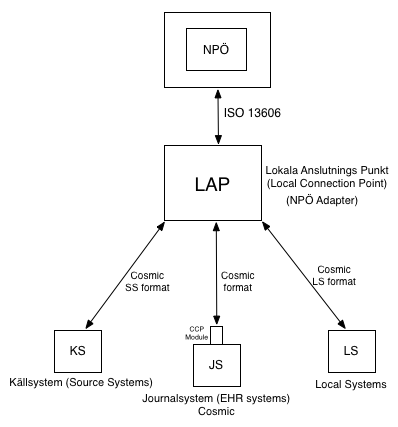
\includegraphics[width=0.55\textwidth]{Images/npoAdapt}
\end{figure}\

\subsection{Solutions}
\label{sec:interopSolutions}
There are two takes on the solution to interoperability that are generally accepted.  Since interoperability is essentially making sure that two or more systems can exchange information, the two most popular solutions are to either make sure that all systems are capable of using the same data formats (Syntactic) or there exists some way for the systems to automatically interpret other data formats used that they do not support (Semantic).

Of course, each of these solutions comes with both advantages and disadvantages.  While semantic interoperability might be quicker and less work at first, it is not practical if the number of systems is going to be expanded because then the automation process must be updated every time a new format is added.  Additionally, implementing semantic interoperability only requires that you know the output of the system for the changes to be made while syntactic interoperability requires complete knowledge of the workings of the system as a whole for the changes to be made.  In return, syntactic interoperability is more work up front but does not require any of the existing systems to be modified when new systems are added.

\subsection{Prerequisites for International Interoperability}

To achieve European wide solutions for cross-border transfer of patient information certain requirements need to be fulfilled. There has to be an agreement on the definitions of data sets for both patient summaries and e-prescription, a legal framework for data transfer, a technical framework to connect the systems at each level, and a working semantic \gls{interoperability}. \cite{epSOS1}
\label{sec:interopPrereq}

\subsection{Care plans}
\label{sec:interopPlans}
%Lastly, care plans will be described and it will be discussed how standardizing them could potentially help the interoperability of \gls{EHR} systems
%TODO: Add bibliography entry and use it in the other parts of the report
In health care, nursing care plans are used to prioritize diagnoses, set up goals and decide on nursing interventions. Preferably, a classification system is used to improve consistency of terminology. Care plans are also being used within social services to clarify purpose, duration, needs and planned actions within inpatient care of young people. In Sweden this is required by law \cite{SocialServices}.

There is an initiative from \gls{CeHis} to standardize these care plans at a national level in Sweden, to support equal care and patient safety. Preceded by research on the feasibility of a national information structure, the purpose is to to define use cases, clarify and verify the applications of standardized care plans compared to the currently existing local ones \cite{CeHis}.

If NPÖ would adapt to the idea of standardized care plans then it might not only help with the semantic interoperability but also in increasing NPÖs impact on the effectiveness of HCP work routines, thereby increasing the overall benefit of the system at a regional level. \cite{Cambio}

Designing EHR systems to encourage the users to follow standardized care plans increases interoperability. When using a standardized care plan, the user needs to document only the deviations from the plan and the small amount of data relevant to them such as observations. The documentation process should be as automated as possible, to enable the health care professional to devote more time to the patient instead of administrative work. This also reduces the tendency of medical staff documenting for their own sake instead of for the one that will treat the patient next. \cite{Cambio}

\newpage

\section{Technical Standards}
\label{sec:TechnicalStandards}

\subsection{What is a Technical Standard for Computer Software?}
\label{sec:technicalStandardsWhatIs}
A technical standard is a set of recognized and established requirements about software systems that establishes the ``way things should be done". Standards are responsible for the uniformity of web browsers (although not all browsers strictly conform to the standard), the ability for laptops laptop or tablet to connect wirelessly to any access point, and the ability to connect laptops to almost any projector. Software standards specify aspects of a program such as: the format for data storage, format for data transfer, and data layout. This allow different developers, working for different companies, to develop different software programs while still allowing for \gls{interoperability} between them. Software standards are the foundation for software \gls{interoperability}.

\subsection{The Creation of a Standard}
\label{sec:technicalStandardsCreation}
For different parties (software development companies) to agree on software standards they typically create an organization consisting of representatives from the the various software companies. This gives them a forum to contribute ideas and opinions about making a single, unified standard addressing the data \gls{interoperability} problem that needs to be addressed.

\subsubsection{Examples of Software Standards Organizations}

\newglossaryentry{Simple Object Access Protocol}{name = {Simple Object Access Protocol}, description = {is a protocol specification for exchanging structured information in the implementation of Web Services in computer networks}}

\newacronym[\glsshortpluralkey = SOAPs, \glslongpluralkey = Simple Object Access Protocol]{SOAP}{SOAP}{\gls{Simple Object Access Protocol}}

\newglossaryentry{Hypertext Transfer Protocol}{name={Hypertext Transfer Protocol}, description={a networking protocol for distributed, collaborative, hypermedia information systems}}

\newacronym[\glsshortpluralkey=HTTPs ,\glslongpluralkey= Hypertext Transfer Protocol]{HTTP}{HTTP}{\gls{Hypertext Transfer Protocol}}

\newglossaryentry{Extensible Markup Language}{name={Extensible Markup Language}, description={a set of rules for encoding documents in machine-readable form}}

\newacronym[\glsshortpluralkey=XLMs ,\glslongpluralkey=Extensible Markup Languages]{XML}{XML}{\gls{Extensible Markup Language}}

\newacronym[\glsshortpluralkey=HTML ,\glslongpluralkey= Hyper-Text Markup Language]{HTML}{HTML}{Hyper-Text Markup Language}

\newacronym[\glsshortpluralkey=IETFs ,\glslongpluralkey= Internet Engineering Task Forces]{IETF}{IETF}{Internet Engineering Task Force}

\newglossaryentry{World Wide Web Consortium}{name={World Wide Web Consortium}, description={An international group responsible for web standards such as \gls{HTML}, \gls{HTTP}, and \gls{XML} networking protocol for distributed, collaborative, hypermedia information systems}}

\newacronym[\glsshortpluralkey = W3C, \glslongpluralkey = World Wide Web Consortium]{W3C}{W3C}{\gls{World Wide Web Consortium}}

\begin{itemize}
\item \gls{W3C} - Responsible for web standards such as \gls{HTML}, \gls{HTTP}, and \gls{XML} 
\item Institute of Electrical and Electronics Engineers Standards Association (\gls{IEEE} Standards Association) - Responsible for a wide range of standards for engineering such as the 802.11 standard
\item \gls{IETF} - Responsible for providing standards for new Internet related technology 
\end{itemize}

\newacronym[\glsshortpluralkey=FDICs ,\glslongpluralkey= Federal Deposit Insurance Corporations]{FDIC}{FDIC}{Federal Deposit Insurance Corporation}

\subsection{Adherence to Standards}
Adherence to a particular software standard can be either mandatory or voluntary. For example: in the United States banking software must conform to security standards and regulations set forth by the \gls{FDIC}. Any system that does not conform to these standards faces legal action by the United States federal government and as such is not allowed to be used by U.S. banks. On the other end of the spectrum are the standards set forth by the \gls{W3C} as to how a web browser should interpret and render various web pages. These are completely voluntary standards and while most popular, modern browsers conform to a majority of these standards, there are no browsers that achieve complete compliance. They face no legal action for not complying with the \gls{W3C} standards because they are voluntary, not legally mandated.

\subsection{Software Standards and EHR Software}
With the growing ubiquity of the Internet, computers, and modern technology as well as the geographic diversity of medical talent and information, it is doubtless that someday a standard specifying the transmission, storage, and format of electronic healthcare records will be developed; the benefit of such a standard is too great to be ignored. Because patent data is widely varied and medical breakthroughs are discovered daily, any standards regulating \glspl{EHR} will constant revision and modification to stay relevant. Such a standard will require a large international organization to oversee and develop.

\newacronym {IHTSDO}{IHTSDO}{International Health Terminology Standards Development Organization}
\newacronym {SNOMED}{SNOMED CT}{Systematized Nomenclature of Medicine - Clinical Terms}

\newglossaryentry{Health Level 7}{name={Health Level 7}, description={A standard organization focusing on the development of international healthcare informatics interoperability standards}}
\newacronym {HL7}{HL7}{\gls{Health Level 7}}

\newglossaryentry{The International Organization for Standardization}{name={A standard setting organization concerned not only with health informatic standards}}
\newacronym {ISO}{ISO}{\gls{The European Committee for Standardization}}

\newglossaryentry{The European Committee for Standardization}{name={The European Committee for Standardization}, description={Aims to provide infrastructures for the development, maintenance and distribution of coherent sets of standards and specifications in Europe}}
\newacronym {CEN}{CEN}{\gls{The European Committee for Standardization}}

\subsection{Terminology}
\label{sec:TechnicalStandardsTerminology}
In order for interoperability to be useful, everyone reading the \gls{EHR} needs to have a common understanding of the information in it. One way to achieve this is by using a common a standardized clinical terminology system.

\subsubsection{SNOMED CT}

\gls{IHTSDO} is a non-profit organization dealing with standards and at the moment 17 countries are members of the organization; among these is Sweden, the United Kingdom, and the United States of America. \gls{IHTSDO} acquired \gls{SNOMED} in 2007 and made it more accessible for a wider audience. \gls{SNOMED} is currently available in US English, UK English, Spanish, Danish, and Swedish and is being translated into French, Lithuanian, and several other languages as well\cite{ihtsdolang}.

\gls{SNOMED} is built up on 311 000 active concepts and is continuously growing. The basic concept behind \gls{SNOMED} is that each medical term has its own unique ID and all these terms are connected by semantic relationships. On \gls{IHTSDO}s website they describe the relationships like this: One type of link is the “IS\_A” relationship. This is used to define a concepts position within a hierarchy, e.g. Diabetes Mellitus IS\_A disorder of glucose regulation."\cite{ihtsdocomp}. If healthcare information and patient data is structured differently at different \glspl{HCP}, searching for specific data in a patient journal and exporting data to other systems gets harder, \gls{SNOMED} aims to address this problem.

By having unique identifiers for all terms, translation between different languages is possible. Every language has the same identifier on their respective term, so when they store a record it is stored as just numbers. This only happens in the back-end so the user will see the medical record written in their own language.

\gls{SNOMED} is centrally updated twice a year where they add new terms and set some terms inactive. In order to support previous versions they never delete terms, but instead mark them as inactive and suggest using the newest term.%\cite{annavik}

\subsubsection{The HL7, ISO and CEN standards}
\gls{HL7}, \gls{ISO} and \gls{CEN} are the main health informatic standards development organizations. They have developed HL7 version 3 and \gls{EN13606} which are meant to supplement the \gls{SNOMED} standard in providing prerequisites for \gls{EHR} \gls{interoperability}.

HL7 version 3 and \gls{EN13606} form one step in accomplishing national information structures. From the interview with Johan Thorwid \cite{Cambio} we learned that the HL7 v2.3 is hard to implement and incomplete due to the additional support information needed for the application to be truly useful. HL7 3.0 was designed with the aim of dealing with this issue – it was supposed to support all healthcare workflows. Among other things, it uses concepts similar to the archetypes and templates of openEHR and specifies different communication formats, but was never adopted in Sweden. In Sweden \gls{EN13606} is used instead. HL7 version 3 is however used in England \cite{Cambio} and within epSOS \cite{epSOS}.

\subsection{Ideal EHR Standard}
All medical institutions have different needs and demands which often very significantly. This makes it exceedingly difficult to create a "one-size fits all" \gls{EHR}. An ideal \gls{EHR} standard will follow the trend of historically successful interfaces and will closely replicate the old paper version. It would also store the records in a standardized format as this maximizes interoperability and data mobility but also allows for the interfaces to the system to be customized for a specific institution. Customizing each \gls{EHR} for a specific institution adds overhead development and maintenance costs but maximizes the work flow productivity at each facility while maintaining interoperability. 

\subsection{An Alternative to a Future EHR Standard}
\label{sec:TechnicalStandardsAlternative}
The only other option that achieves interoperability for sharing healthcare records would be a single unified software system that doctors all over the world would use to view and modify patient records. Such a solution is unrealistic for two reasons: there are already too many \gls{EHR} software companies to reasonably plan for one new company to globally take over the entire \gls{EHR} industry, and with anti-trust laws as well as fair competition clauses in many countries (such as the United States and Sweden) a single organization would not be legally allowed to be the sole producer of \gls{EHR} software systems.

\newpage

\section{Adoption of Future Systems}
\label{sec:Future}

\subsection{Technical Limitations}

The technical limitations for an \glspl{EHR} system are multi-faceted. Two separate approaches to a solution are outlined in the United States’ Department of Health and Human Services paper Health Information Technology: Initial Set of Standards, Implementation Specifications, and Certification Criteria for Electronic Health Record Technology. \cite{AMA} 

One solution is to use \gls{SOAP} which is a specification for exchanging structured information. This setup relies on \gls{XML}, a remote procedure call, and \gls{HTTP}. Significant existing software infrastructure and development already exists and SOAP is a way to re-use that has already been done. This solution is dependent on multiple different systems and if one of the needed layers malfunctions the system as a whole will stop working. 

Additionally, because \gls{XML} formatted data is used, \glspl{SOAP} systems are usually slower and more data-heavy than other options. This might cause a scalability problem for a large system. These limitations to the design may cause future problems implementing a \glspl{SOAP} style system on a large scale.

\gls{SOAP} is a trade-off however: the ability to work practically everywhere and stand on top of hundreds of existing standards comes with significant overhead and additional complexity. Very few other systems, however, have the ability to deal with data as complicated as what is found in \glspl{EHR}
\label{sec:futureTechnical}
\subsection{Legal Issues}

The new Swedish legislation provides new opportunities, but not obligations. \cite{RiR19}

\glspl{EHR} exist to promote patient safety, high quality health care and minimized cost. It is also supposed to be a source of information for the patient (ch 3, § 2). A patient journal must be kept for each patient and may not be common to several patients. The one writing in the journal is responsible for that part. All journal entries must be written in Swedish. \cite{PatientDataAct}

The patient is not required to give his or her consent for the \gls{HCP} to act according to what the Patient Data Law dictates, except for an \gls{EHR} to be shared from one caregiver to another, when gaining electronic access to records of another care unit or during unified journaling. Patients may refuse to be part of organized records (kvalitetsregister). To remove parts of a journal there needs to be convincing reasons, the part being removed can't be necessary for future health care, and there should be no public interest in keeping the information. Journal data may be blocked from unified journaling access but the information saying that data has been blocked and by who should still be available. 

A caregiver may only have access to documented information if they directly participate in the care of the patient or need this information for their work in health care. The law also regulates periodic checking of the logs. The patient has rights to obtain certain parts of their medical journal and information on who has accessed it in the past.\cite{PatientDataAct}

The Personal Data Privacy Act (1998:204) applies to the parts of the records that are managed automatically and stored in a structured fashion. The National Board of Health and Welfare has rights and obligations regarding apprehension of journals in the event of legal violations.\cite{PatientDataAct}

According to the Swedish Patient Safety Act (2010:659), a caregiver must immediately inform a patient who has suffered a medical injury about the injury, planned preventive measures, complaint and compensation
options and the patient councils activity. Information on the information provided shall be recorded in the patient record.\cite{PatientSafetyAct}

If, with regard to the purpose of ongoing health care, it is of considerable importance that the data is not provided to the patient, then the caregiver is not allowed to do so. The same applies if there is risk of violence or permanent damage to the patient should the information be disclosed. Unless required to by law, a caregiver is not allowed to disclose details of health or personal conditions about a patient to outsiders.\cite{PatientSafetyAct}
\label{sec:futureLegal}
\subsection{Organizational Issues}
%[Emil and Erik: Current organizational issues that limit the adoption of interoperating systems.]
In order to successfully implement a new system for \gls{EHR} sharing all the layers of the organizational effort must be involved~\cite{Empirica} including doctors, nurses, administrators, etcetera. Since this will change the way people work and what responsibilities they have~\cite{Empirica} everyone involved must commit to the system change effort in order for the switch to go well.

In order to get all layers of the organization interested in the integration process it is important to involve them in the development of the system~\cite{Empirica}. Instead of having just the managers talking to the developers, all of the layers should be involved in the development stage of the system so that they feel like they have a say about the system that they will eventually use.

When developing \gls{EHR} systems it is important to have clear objectives, ability to continuously revise, and most importantly strong project leaders with the backing of top level management and politicians~\cite{Empirica}. This ties in to the previous topic of having all the layers of the organization involved in the development of the system. When implementing new features or changing existing ones developers need to ensure that they listen and understand what users want. Users are seldom completely certain of exactly what they want and that makes it easy to make changes based on misunderstandings.
\label{sec:futureOrganizational}
\subsection{Usability Issues}
%[Romel: One problem is to identify the people responsible for the systems usability.]
The aim of establishing a successful \gls{EHR} system is to improve efficiency, effectiveness, and support the clinicians in their practice to perform high quality care. Clinical professions have different clinical practices and use the system differently. This can cause problems because some of them feel the system does not support their clinical practice. Usability has thus been cited as a major factor in both acceptance and effectiveness of \gls{EHR}s in the clinical settings. Some of the key usability issues in EHR are listed below:
\begin{itemize}
\item Not intuitive - lack of patient overview especially for the physicians
\item Many clicks - cumbersome navigation
\item Time consuming - response time e.g. downloading list of tab results can take minutes if a patient have many tests
\item Does not support work routines - flaws in design leading to threatening situations:  e.g. unclarity about dosage in the  prescription module.
\end{itemize}

There are many potential reasons for this lack of attention on \gls{EHR} usability. One problem is to identify the people responsible for the systems usability. Janols et al [?] had examined how a large Swedish county with several healthcare units works with usability problems in the \gls{EHR} [?] deployment process. They showed that there is confusion about the responsibility for usability issues with the organization. The confusion is because some of the stakeholders consider the\gls{EHR} system to be an IT system, not an integral part of the healthcare process. Others consider it to be a core business system and therefore the core business responsibility. This confusion and uncertainty about responsibility leads to an unsustainable work situation for the care staff that needs an effective \gls{EHR} system to perform a high quality work.
\label{sec:futureUsability}
%Here are related items from the Empirica interview
%\begin{itemize}
%\item When it comes to \gls{interoperability}, technical issues and standard specifications are subordinated to legal and organizational %issues. The organizational issues include common understanding from people involved in the process and getting the commitment from %doctors and nurses. 
%\item Clear objectives and strong project leaders with the backing of the top level management and politics are very important factors of %success for \gls{EHR} projects. Continuous development and the ability to revise things are also crucial.
%\item It is important to reach all the layers of the health care organization to achieve change, to engage the different groups of doctors, %nurses, secretaries, technicians and not only have the software developers talk to the management section of the organization.
%\item Electronic systems are changing the way doctors work and what responsibilities they have.
%\end{itemize}

\newpage

\section{Results/ Discussion}
\label{sec:Results}

\subsection{Prerequisites for increased interoperability}
\label{sec:resultsPrereq}
\subsection{Types of solutions and implications for the end user}
\label{sec:resultsEndUser}
\subsubsection{Integrated vs. Standalone Application}
When designing an interoperating EMR system the choice is either whether integrate interoperating functionality into the existing EHR application or to create a standalone solution capable of retrieving all information available about a patient.

A standalone system could be implemented either as a desktop application or in a web application. From a usability perspective a standalone application could cause a few usability issues. The standalone solution does not take advantage of the users knowledge of the legacy system as they have to learn a new user interface specific for the interoperating system. A workaround for this could be to allow individual hospitals to customize the end user interface to accommodate differences in user needs. 
Another issue is that a standalone application forces the end user to multi-task between the legacy \gls{EHR} system and the new interoperating application. This increases the complexity of the work environment as it does not take advantage of cognitive abilities available to humans, and adds an additional burden on the memory. 

A solution integrating into the existing \gls{EHR} systems on the other hand takes advantages of what the user already knows, decreasing the need for them to change their behavior patterns. The user can do all the work in the system they are currently using.

There might still be need for changes in the existing systems as they way information is handled need to conform to common semantic standards. This would render changes both in the end user interface and the behavior of how they interact with the system. Integrating interoperability into existing systems does not increase the end users need for multitasking or burdens the short-time memory. It also supports diversification in the end user interfaces encouraging competitiveness and customization.

\subsubsection{Standards}
\label{sec:resultsStandards}
To make a system that interoperate between different \gls{EHR} systems a standard have to be set and forced onto the systems. This standard creates means for the \gls{EHR} systems to share data in a way that all the systems can interpret and handle it. There are several standards currently in development.

Before sending the data to other \gls{EHR} systems, an interface or adapter is needed to transform the data into a set standard. NPÖ uses an adapter to translate information from the originating systems into a set of common standards. 

One of the problems with implementing a system like this is getting all the systems to unite and accept and use a set standard. To be able to make this work the different systems need to use the same semantics and therefore some users may have to change the way they are editing data in the \gls{EHR} system. The interface of the systems also might be forced to change the way information is entered and presented to conform to specific semantics and standards. Some \gls{EHR} systems will be more affected by the standard than others, and will therefore have to change more.

\subsubsection{Data Locality}
\label{sec:resultsLocality}
\newacronym[\glsshortpluralkey=HCUs ,\glslongpluralkey= Health Care Units]{HCU}{HCU}{Health Care Unit}

To achieve interoperability in a \gls{EHR} system patient information has to be made available throughout all connected health care units. This raises a few concerns regarding the ownership of data, and who actually controls the data and keeps track of existing copies etc. The information could either be kept in a centralized or decentralized manner.

Keeping the data centralized will require large amounts of data storage and intensive traffic between the connected health care units. The amount of data to be kept centrally can be reduce as up to 60\% of the storage at local hospitals are used for version tracking. Storing the data centrally could also decrease the search and retrieval time for accessing a health record as the information is kept closer to each individual \gls{HCU}.
%source: interview with Johan Thorwid.
Allowing patient information to be stored centrally will also require that \gls{HCU} allows giving up some of their control over the data. The system should be implemented with the possibility for \glspl{HCU} to remove information available in the central domain upon patient requests. Another issue would be to ensure that data is consistent between individual health-care units updating information about patients and the central system. An implemented system has to ensure that new information is updated to the central system within acceptable time.

On the other hand a decentralized system where the information is kept at each individual health-care unit allows higher control of the patients information. When requested by a secondary \gls{HCU} the information will only reside outside of the system for a temporary time. There would still be a need for centrally indexing where information is available to avoid flooding hospitals with requests for patient information. A benefit from having a decentralized system is that it to some extent guarantees that the retrieved information is up to date as it is retrieved upon access.

\subsubsection{Personal Health Records}
\label{sec:resultsPHR}
A possible addition to a system like this could be to implement an interface for patients to access their Personal Health Records from their home computers. This would be a useful way for patients to obtain the various medical records that are shown to schools, employers, or whoever they may need to share medical information with. Additional beneficial features could also be implemented into the health records to extend its functionality with self-care functionality and allow patients to carry out preliminary test before visiting their health care unit. \glspl{PHR} become a sensitive issue as it means making patient records available on the Internet.

\subsection{Security}
\label{sec:resultsSecurity}
The system needs to be secure, no unauthorized users should be able to access data. Different levels of security can be used but a standard of security level for authentication in the system must be set. In a integrated system the users are using the \gls{EHR} systems, where they have authentication to able to access information, all that is needed is that every EHR system fulfill the required standard for security. In a standalone system the system itself will have the meet the same requirements as the existing \gls{EHR} systems. 
The communication in the system could be kept in a intranet or on the Internet. If a intranet is used the security will be higher and less or no encryption will be needed. However if intranet is used there could be complications when implementing a \gls{PHR} system as you would need to get access to the intranet somehow via Internet.

\subsubsection{Requirement Domains}
Deploying an interoperating system requires the involved health care providers to agree on communicating in specific ways. This will render a set of requirements to be forced on each hospital. These requirements can be divided into different domains depending on their importance. For example how to communicate with the central system would be a mandatory requirement. Other requirements could be recommended or optional, giving the individual hospitals guidance and a higher degree of freedom for how to implement an \gls{EMR}.

The system also has to be secure, no unauthorized users should be able to access data. As the users are using the old \gls{EHR} systems, where they have authentication to able to access information, all that is needed is that every \gls{EHR} system fulfill a required standard for security. The whole system can also be kept in a intranet to avoid intrusion even further.

\subsection{Recommended Development Methodologies}
The interviews with administrative personal and technicians were focused on what they thought would be required to create interoperability between \glspl{EHR} rather than what they would want in such a system. 

One of the most important things learned from these interviews was that the development of an interoperable system would be very complex. It is hard to define a definite end in such a big development process and the process should be considered on-going where focus lie on completing sub-goals rather than only shooting for the final goal. In other words the work should be approached with a type of agile development. 

\subsubsection{AGILE}
Agile development is an iterative and incremental development process where the work is done in small steps and every step is evaluated. The small steps could be subparts of the final system. Starting off with a smaller part of the system, ensuring that this part works and then move on by adding more features or go on to the next part of system might be more successful than trying to complete the whole system at once. However, this could be very time consuming and is not an option if there is a short amount of time to complete the system. It is therefore important to consider the amount of time and resources that can be spent on the project against the size of the iterative steps in the agile development.

\subsubsection{Usability Testing}
\label{sec:resultsUsabilityTesting}
Another important aspect that came up during the interviews was the involvement of the end-user in the development process. The end-user in an interoperable system between \glspl{EHR} is the users of the \glspl{EHR} such physicians, nurses etc. If the development of the interoperable system can not be done only in the back-end, meaning that the end-user's systems will be affected, their opinions will be of importance. In this case the change in the systems might be made in a way that does not affect the end-users negatively if their opinions are taken into consideration in the development. Even if there is no need for noticeable changes their opinions can still be of importance when it comes to what kind of patient information that is most important to share in the interoperable system if it is unmanageable to share all information. 

The involvement of end-users can be included in the agile development by letting them take part in the evaluation of the sub-parts where their opinions matter. 

\subsubsection{Security Testing}
During the interviews the issue regarding security came up as an important factor to consider in an interoperable system. It is always important to handle the security with great care when it comes to patient information, but the security issues might be a lot greater when dealing with a system of bigger size such as when multiple \glspl{EHR} is interoperating. One example of a feature that might need improvement is the access control of patient information due to the fact that an interoperable system will increase the amount reachable information. Ordinary methods for checking access control such as going through logs might be inefficient and costly and new methods might be needed.

\subsubsection{Feasibility}
One of the problems with implementing a system like this is to get all the systems to unit and accept a set standard to be used. Some of the systems has to change more then others.
Having a large central database for all \gls{EHR} data (Sweden) could be considered hard to manage but according to Johan Thorvid it should be feasible.

\subsubsection{Usability Implications}
This integrated solution is supposed to have as small implication as possible for the users. There might be some small changes as the systems that they are currently using may have to change a bit to be able to meet the standards that are going to be used. As the semantics has to match some of the users may have to change how they write. However with a integrated solution the user can do all the work in the system they are currently using. Most of the old systems will however still be intact and the users can use the old knowledge and experience when navigating.

\newpage

\section{Conclusions}
\label{sec:Conclusions}



\newpage
\printglossaries
\newpage

\begin{appendix}
\end{appendix}



\bibliographystyle{unsrt} 
\bibliography{ourBib} 

\end{document} 
